\section{Durchführung}
\label{sec:Durchführung}
\subsection{Aufbau}
\begin{figure}
  \centering
  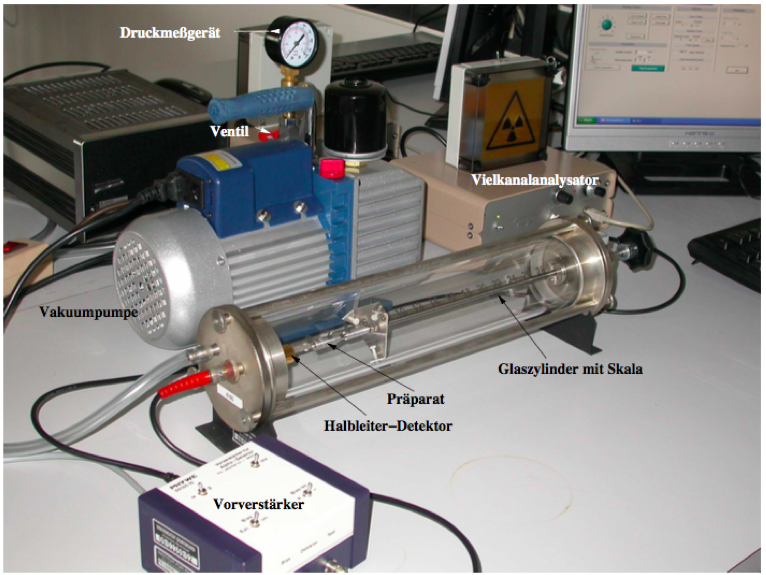
\includegraphics[width=11cm]{Aufbau.png}
  \caption{Versuchsaufbau \cite{skript}.}
  \label{fig:aufbau}
\end{figure}
Der Aufbau des Versuchs ist in Abbildung \ref{fig:aufbau} dargestellt.
Die $\alpha$-Quelle, in diesem Fall ein Am-Präparat, befindet sich
in einem Glaszylinder, welcher durch eine Vakuumpumpe evakuiert werden kann.
Das Präparat zerfallt nach der Zerfallsgleichung
\begin{equation}
  \ce{^{241}_{95}Am -> ^{237}_{93}Np + ^{4}_{4}He^{++}} \:,
  \label{eqn:reak}
\end{equation}
mit einer Halbwertszeit von $\text{T}_{1/2}= 458$a.\\
Am Ende des Glaszylinders befindet sich ein Halbleiter-Sperrschichtzähler, welcher
als Detektor fungiert. Dieser ist im Prinzip wie eine in Sperrrichtung betriebene
Diode aufgebaut, sodass die einfallenden $\alpha$-Teilchen Elektronen-Loch-Paare
erzeugen, deren durch einen Vorverstärker verstärkte Stromimpulse in einem
Vielkanalanalysator registriert werden. Die Messung wird in einem Histogramm ausgegeben,
wobei die Pulshöhe proportinal zur Energie der $\alpha$-Strahlung ist.
Der Abstand zwischen Detektor und Quelle lässt sich bei diesem Aufbau variieren, da das
Präparat auf einem verschiebbaren Halter angebracht ist.
\subsection{Bestimmung der Reichweite}
Zunächst wird die Verkabelung des Aufbaus überprüft, wobei die eventuellen Korrekturen
am Sperrschichtzähler nur ohne anliegende Spannung durchgeführt werden dürfen.\\
Der $\alpha$-Strahler wird nun auf einem festen Abstand fixiert und mithilfe der Vakuumpumpe
wird nun der Glaszylinder evakuiert bis der Druck auf etwa
$p \approx 0$ gesunken ist.
Anschließend wird im Computerprogramm der $Acqusition Mode$ auf $Auto$
gestellt und eine Messzeit von 2 Minuten eingestellt. Nach Beendigung der Messung wird
die gesamte Zählrate, sowie die Position des Energiemaximums notiert.
Der Druck wird dann in Abständen von $\SI{50}{\milli\bar}$ erhöht und die Messung jeweils
wiederholt.\\
Die gesamte Messung wird im Anschluss mit einem anderen Abstand erneut
durchgeführt.
\subsection{Statistik des radioaktiven Zerfalls}
Zur Überprüfung der Statistik des radioaktiven Zerfalls wird an der Apparatur ein
fester Abstand eingestellt, der Zylinder vollständig evakuiert und die Messzeit auf $\SI{10}{\second}$ gesetzt. Nun werden
mindestens 100 Messungen durchgeführt, bei denen jeweils die Anzahl der Zerfälle notiert
werden.
